%%%%%%%%%%%%%%%%%%%%%%%%%%%%%%%%%%%
%This is the LaTeX ARTICLE template for RSC journals
%Copyright The Royal Society of Chemistry 2016
%%%%%%%%%%%%%%%%%%%%%%%%%%%%%%%%%%%

\documentclass[twoside,twocolumn,9pt]{article}

\usepackage{tgheros}
\renewcommand{\familydefault}{\sfdefault}

\usepackage{extsizes}
\usepackage[super,sort&compress,comma]{natbib} 
\usepackage[version=3]{mhchem}
\usepackage[left=1.5cm, right=1.5cm, top=1.785cm, bottom=2.0cm]{geometry}
\usepackage{balance}
\usepackage{mathptmx}
\usepackage{sectsty}
\usepackage{graphicx} 
\usepackage{lastpage}
\usepackage[format=plain,justification=justified,singlelinecheck=false,font={stretch=1.125,small,sf},labelfont=bf,labelsep=space]{caption}
\usepackage{float}
\usepackage{fancyhdr}
\usepackage{fnpos}
\usepackage[english]{babel}
\addto{\captionsenglish}{%
  \renewcommand{\refname}{Notes and references}
}
\usepackage{array}
\usepackage{droidsans}
\usepackage{charter}
\usepackage[T1]{fontenc}
\usepackage[usenames,dvipsnames]{xcolor}
\usepackage{setspace}
\usepackage[compact]{titlesec}
\usepackage[utf8]{inputenc}
\usepackage{physics}
\usepackage[mathscr]{euscript}  % \mathscr

%%%Please don't disable any packages in the preamble, as this may cause the template to display incorrectly.%%%


\usepackage{xcolor}
\definecolor{ugent_blue}{RGB}{30, 100, 200}
\definecolor{ugent_yellow}{cmyk}{.0, .10, 1, 0}

\usepackage{titlesec}
\titleformat{\section}
{\color{ugent_blue}\normalfont\Large\bfseries}
{\color{ugent_blue}\thesection}{1em}{}

\usepackage[colorlinks=true,linkcolor=black,citecolor=ugent_blue]{hyperref}
\usepackage{cleveref}

\usepackage{lineno}
\linenumbers

%\AtEveryCite{\color{ugent_blue}}




\usepackage{epstopdf}%This line makes .eps figures into .pdf - please comment out if not required.

\definecolor{cream}{RGB}{222,217,201}

\begin{document}

\pagestyle{fancy}
\thispagestyle{plain}
\fancypagestyle{plain}{
%%%HEADER%%%
\renewcommand{\headrulewidth}{0pt}
}
%%%END OF HEADER%%%

%%%PAGE SETUP - Please do not change any commands within this section%%%
\makeFNbottom
\makeatletter
\renewcommand\LARGE{\@setfontsize\LARGE{15pt}{17}}
\renewcommand\Large{\@setfontsize\Large{12pt}{14}}
\renewcommand\large{\@setfontsize\large{10pt}{12}}
\renewcommand\footnotesize{\@setfontsize\footnotesize{7pt}{10}}
\makeatother

\renewcommand{\thefootnote}{\fnsymbol{footnote}}
\renewcommand\footnoterule{\vspace*{1pt}% 
\color{cream}\hrule width 3.5in height 0.4pt \color{black}\vspace*{5pt}} 
\setcounter{secnumdepth}{5}

\makeatletter 
\renewcommand\@biblabel[1]{#1}            
\renewcommand\@makefntext[1]% 
{\noindent\makebox[0pt][r]{\@thefnmark\,}#1}
\makeatother 
\renewcommand{\figurename}{\small{Fig.}~}
\sectionfont{\sffamily\Large}
\subsectionfont{\normalsize}
\subsubsectionfont{\bf}
\setstretch{1.125} %In particular, please do not alter this line.
\setlength{\skip\footins}{0.8cm}
\setlength{\footnotesep}{0.25cm}
\setlength{\jot}{10pt}
\titlespacing*{\section}{0pt}{4pt}{4pt}
\titlespacing*{\subsection}{0pt}{15pt}{1pt}
%%%END OF PAGE SETUP%%%

%%%FOOTER%%%
\fancyfoot{}
\fancyfoot[LO,RE]{\vspace{-7.1pt}
\includegraphics[height=9pt]{head_foot/LF}}
\fancyfoot[CO]{\vspace{-7.1pt}\hspace{11.9cm}
\includegraphics{head_foot/RF}}
\fancyfoot[CE]{\vspace{-7.2pt}\hspace{-13.2cm}
\includegraphics{head_foot/RF}}
\fancyfoot[RO]{\footnotesize{\sffamily{1--\pageref{LastPage} {\color{ugent_yellow} ~\textbar } \hspace{2pt}\thepage}}}
\fancyfoot[LE]{\footnotesize{\sffamily{\thepage~{\color{ugent_yellow} ~\textbar }\hspace{4.65cm} 1--\pageref{LastPage}}}}
\fancyhead{}
\renewcommand{\headrulewidth}{0pt} 
\renewcommand{\footrulewidth}{0pt}
\setlength{\arrayrulewidth}{1pt}
\setlength{\columnsep}{6.5mm}
\setlength\bibsep{1pt}
%%%END OF FOOTER%%%

%%%FIGURE SETUP - please do not change any commands within this section%%%
\makeatletter 
\newlength{\figrulesep} 
\setlength{\figrulesep}{0.5\textfloatsep} 

\newcommand{\topfigrule}{\vspace*{-1pt}% 
\noindent{\color{cream}\rule[-\figrulesep]{\columnwidth}{1.5pt}} }

\newcommand{\botfigrule}{\vspace*{-2pt}% 
\noindent{\color{cream}\rule[\figrulesep]{\columnwidth}{1.5pt}} }

\newcommand{\dblfigrule}{\vspace*{-1pt}% 
\noindent{\color{cream}\rule[-\figrulesep]{\textwidth}{1.5pt}} }

\makeatother
%%%END OF FIGURE SETUP%%%

%%%TITLE, AUTHORS AND ABSTRACT%%%
\twocolumn[
  \begin{@twocolumnfalse}
{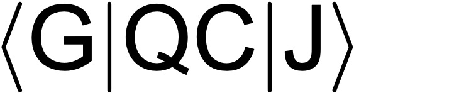
\includegraphics[height=30pt]{head_foot/journal_name}\hfill\raisebox{0pt}[0pt][0pt]{
\includegraphics[height=55pt]{head_foot/RSC_LOGO_CMYK}}\\[1ex]

\includegraphics[width=18.5cm]{head_foot/header_bar}}\par
\vspace{1em}
\sffamily
\begin{tabular}{m{4.5cm} p{13.5cm} }

& \noindent\LARGE{\textbf{Phase transitions in the Bose-Hubbard model$^\dag$}} \\%Article title goes here instead of the text "This is the title"
\vspace{0.3cm} & \vspace{0.3cm} \\

& \noindent\large{Xeno De Vriendt\textit{$^{a}$}, Robbe Brants\textit{$^{b}$}} \\%Author names go here instead of "Full name", etc.

& \\

& \noindent\normalsize{Do \emph{not} write an abstract. That will be done when the outline has matured into a completed paper.} \\%The abstrast goes here instead of the text "The abstract should be..."

\end{tabular}

\end{@twocolumnfalse} \vspace{1.6cm}

  ]
%%%END OF TITLE, AUTHORS AND ABSTRACT%%%

%%%FONT SETUP - please do not change any commands within this section
\renewcommand*\rmdefault{bch}\normalfont\upshape
\rmfamily
\section*{}
\vspace{-1cm}


% %%%FOOTNOTES%%%

\footnotetext{\textit{$^{a}$~Department of Chemistry, Ghent University, Krijgslaan 281 (S3), B-9000 Ghent, Belgium}}
\footnotetext{\textit{$^{b}$~Department of Physics and Astronomy, Ghent University, Krijgslaan 281 (S9), B-9000 Ghent, Belgium}}

% %Please use \dag to cite the ESI in the main text of the article.
% %If you article does not have ESI please remove the the \dag symbol from the title and the footnotetext below.
% \footnotetext{\dag~Electronic Supplementary Information (ESI) available: [details of any supplementary information available should be included here]. See DOI: 00.0000/00000000.}
% %additional addresses can be cited as above using the lower-case letters, c, d, e... If all authors are from the same address, no letter is required

% \footnotetext{\ddag~Additional footnotes to the title and authors can be included \textit{e.g.}\ `Present address:' or `These authors contributed equally to this work' as above using the symbols: \ddag, \textsection, and \P. Please place the appropriate symbol next to the author's name and include a \texttt{\textbackslash footnotetext} entry in the the correct place in the list.}


%%%END OF FOOTNOTES%%%

%%%MAIN TEXT%%%%


\section{Introduction}

The Bose-Hubbard model provides an excellent testbed to study quantum phase transitions (QPTs) \cite{sachdev1999} of strongly interacting bosonic systems in one \cite{kuhner1998} as well as higher dimensions \cite{freericks1994}. Due to the fundamental algebra underlying the physics of bosonic systems, the phase diagram of the bose-Hubbard model becomes more rich than that of its fermionic counterpart \cite{gu2004, deng2006, cozzini2007, chung2021, devriendt2022}. 

Of particular interest is the Mott-Hubbard transition \cite{mott1949}, which in the bosonic model encapsulates a quantum phase transition from a superfluid to a Mott-insulator (MI) \cite{elstner1999, capello2007, cucchietti2007}. In one dimension, this transition agrees with the Berezinskii-Kosterlitz-Thouless (BKT) \cite{kosterlitz1973} scenario of the interaction-driven Mott transition.

\begin{itemize}
    \item In this work we will aim to model the occurring phase transitions in the bosonic Hubbard model. This can be done by means of constrained wavefunction theory, but different approaches will be studied simultaneously.
    \item By doing so we will be able to gain a deeper understanding of the occurring quantum phase transitions, especially the superfluid-MI BKT transition.
    \item Comparison between results from an exact diagonalization approach \cite{zhang2010} and a matrix-product-state (MPS) \cite{perez2006} approach can lead to insights in where the limits of both approaches lie.
    \item Entanglement studies and quantum information theory principles can be applied in order to further characterize the obtained QPTs.
\end{itemize}

\section{Theory}
\subsection{The bose-Hubbard model}
The bose-Hubbard model Hamiltonian can be defined in an abstract site basis consisting of $L$ sites, allowing for inter-site hopping between nearest neighbors only, while introducing a site-dependent on-site repulsion that penalizes multiple occupation on a single site
\begin{equation}
  \hat{H} = \sum_{<i,j>} t_{ij}\hat{b}_i^\dagger \hat{b}_j + \frac{1}{2}\sum_i U_i\hat{b}_i^{\dagger 2} \hat{b}_i^{2} \thinspace ,
\end{equation}
where $t_{ij}$ is the hopping parameter which only affects nearest neighbors $<i,j>$, $U_i$ is the on-site energetic penalty and $\hat{b}^\dagger$ and $\hat{b}$ are the bosonic creation and annihilation operators respectively, which satisfy the bosonic commutation rules. Oftentimes a site-specific on-site potential is added to this model to allow for the introduction of asymmetry between the sites
\begin{equation}
  \hat{H} = \sum_{<i,j>} t_{ij}\hat{b}_i^\dagger \hat{b}_j + \frac{1}{2}\sum_i U_i\hat{b}_i^{\dagger 2} \hat{b}_i^{2} + \sum_i \omega_i \hat{b}_i^\dagger \hat{b}_i \thinspace .
  \label{eq:bose-hubbard-hamiltonian}
\end{equation}
Since the Hubbard Hamiltonian commutes with the total number operator $\hat{n}$
\begin{align}
  \hat{n}_i = \hat{b}_i^\dagger \hat{b}_i \thinspace &, \\
  \hat{n} = \sum_i \hat{n}_i \thinspace &, \\
  [\hat{H}, \hat{n}] = 0 \thinspace &,
\end{align}
the eigenstates of the Hamiltonian can be expanded in the orthonormal basis spanned by the eigenstates of the number operator
\begin{equation}
    \ket{\Psi}=\sum_{n_{1}\dots n_{L\alpha}} 
    \Psi^{n_{1} \ldots n_{L}}
    \ket{n_{1}\dots n_{L}} 
    \thinspace ,
    \label{theory:eigenstate}
\end{equation}
with $\Psi^{n_{1} \ldots n_{L}}$ the expansion coefficient belonging to a basis state $\ket{n_{1}\dots n_{L}}$ over $L$ sites.

\subsection{ground state properties of the Bose Hubbard model}
Single particle excitations in the groundstate of the Bose-Hubbard model can be defined as the difference between the potentials for half band filling and one particle less than half band filling
\begin{align}
  \mu^+(L) &= E_0(L, N+1) - E_0(L, N) \thinspace ,\\
  \mu^-(L) &= E_0(L, N) - E_0(L, N-1) \thinspace ,
\end{align}
with $E_0(X, Y)$ representing the groundstate energy of the system containing $X$ sites and $Y$ bosons. The excitation gap is then subsequently defined as their difference
\begin{equation}
  \Delta(L) = \mu^+(L) - \mu^-(L) \thinspace .
  \label{eq:gap}
\end{equation}

\subsection{Population redistributions on the bose-Hubbard model}
As shown in literature \cite{devriendt2021, devriendt2022}, we can redistribute particles within our system by imposing constraints through a Lagrangian formalism \cite{mukherji1963, zeiss1983, kaduk2011}
\begin{equation}
  \mathscr{L}(\vb{p}, \mu)
        = E_{tot}(\vb{p})
        - \mu ( m(\vb{p}) - M )
        \thinspace ,
\end{equation} 
where $m(\vb{p})$ is the value of the feature operator at the model parameters $\vb{p}$ and $M$ is the target value for the feature operator. The stationary condition of the Lagrange multiplier $\mu$ yields the value of the defined feature operator, and the stationary conditions of the model parameters $\vb{p}$ can be written as
\begin{equation}
  \eval{
    \pdv{
        \mathscr{L}(\vb{p}, \mu)
    }{p_i}
}_{\mu^\star, \thinspace \vb{p}^\star}
= \eval{
    \pdv{
        E_{tot}(\vb{p})
    }{p_i}
}_{\vb{p}^\star}
- \mu^\star \qty( 
    \eval{
        \pdv{
            m(\vb{p})
        }{p_i}
    }_{\vb{p}^\star}
)
= 0
\thinspace .
\label{eq:stationary_condition_model_parameters}
\end{equation}
Using these stationary conditions we can derive a modified Hamiltonian $\hat{H}_{mod}(\mu)$ where the feature operator $\hat{m}$ is weighed by the value of the Lagrange multiplier
\begin{equation}
  \hat{H}_{mod}(\mu) = \hat{H} - \mu \hat{m} \thinspace .
  \label{eq:modified-hamiltonian}
\end{equation}
It is important yto note that, while the modified Hamiltonian is suited to optimize the model parameters of the wave function in such a way that the stationary condition of the Lagrange multiplier is satisfied, the energy of the system needs to be calculated using the original Hamiltonian of the system. This can be achieved by correcting for the imposed feature
\begin{align}
  \begin{split}
    E_{tot}(\vb{p}^\star)
    &= \ev*{\hat{H}}{\Psi(\vb{p}^\star)} \\ 
    &= \ev*{\hat{H}_{\text{mod}} + \mu\hat{m}}{\Psi(\vb{p}^\star)}
    \thinspace .
  \end{split}
\end{align}
In the context of the bose-Hubbard model, we will construct a feature operator with the goal of imposing bosonic redistributions on our model system. This can be done by arbitrarily dividing the total lattice into an \emph{open subsystem} $\Omega_{os}$ and an \emph{environment} $\omega_{env}$
\begin{equation}
  \Omega = (\Omega_{os}, \Omega_{env}) \thinspace ,
\end{equation} 
and subsequently defining the feature operator as the number operator of the open subsystem
\begin{equation}
  \hat{m} = \sum_i^{os}\hat{n}_i \thinspace .
  \label{eq:feature}
\end{equation}
Combining \cref{eq:modified-hamiltonian} with \cref{eq:bose-hubbard-hamiltonian} and \cref{eq:feature} yields
\begin{equation}
  \hat{H}_{mod}(\mu) = \sum_{<i,j>} t_{ij}\hat{b}_i^\dagger \hat{b}_j + \frac{1}{2}\sum_i U_i\hat{b}_i^{\dagger 2} \hat{b}_i^{2} + \sum_i \omega_i \hat{b}_i^\dagger \hat{b}_i - \sum_i^{os}\hat{n}_i \thinspace ,
\end{equation}
where the \emph{chemical potential} $\mu$ can be tuned in order to impose a certain redistribution of bosons between the open subsystem and the environment.

\section{Methodology}

For the exact diagonalization (ED) calculations we look at a one-dimensional bose-Hubbard model of three sites, in the number sector where our system contains three bosons. The ED algorithm is self-implemented based on the algorithm described by Zhang and coworkers \cite{zhang2010}. $U/t$ is varied by gradually lowering the nearest neighbor hopping $t_{ij}$, evolving the system towards a more strongly correlated state. The formalism of constraints is either applied by scanning over a range of chemical potentials ($\mu_{os}$) or by optimizing the Lagrange multiplier in order to impose a certain population on the open subsystem ($N_{os}$). The latter is achieved by finding the root of the associated constraint $(\hat{n} - \expval{\hat{n}})$. When optimizing towards a certain population, a small asymmetry is introduced in the on-site potentials $\omega_i$, in order to facilitate the optimization procedure. For larger systems, the ITensors package \cite{Fishman2022} density matrix renormalization group (DMRG) algorithm was used.

\section{Results and discussion}
\subsection{Population redistributions show the effects of Mott-Hubbard type transitions}
The chemical potential $\mu_{os}$ induces changes in the open subsystem population $N_{os}$, which becomes increasingly stepwise as $U/t$ is increased, leading to the appearance of \emph{Mott-Hubbard plateaus} (\cref{fig:Mott-Hubbard}). The applied chemical potential determines when a given boson is exchanged between the open subsystem and its environment. While at low $U/t$-values, this process occurs continuously, the more strongly correlated the system becomes, the more discontinuous the exchange process becomes. 
\begin{center}
    \begin{figure}
        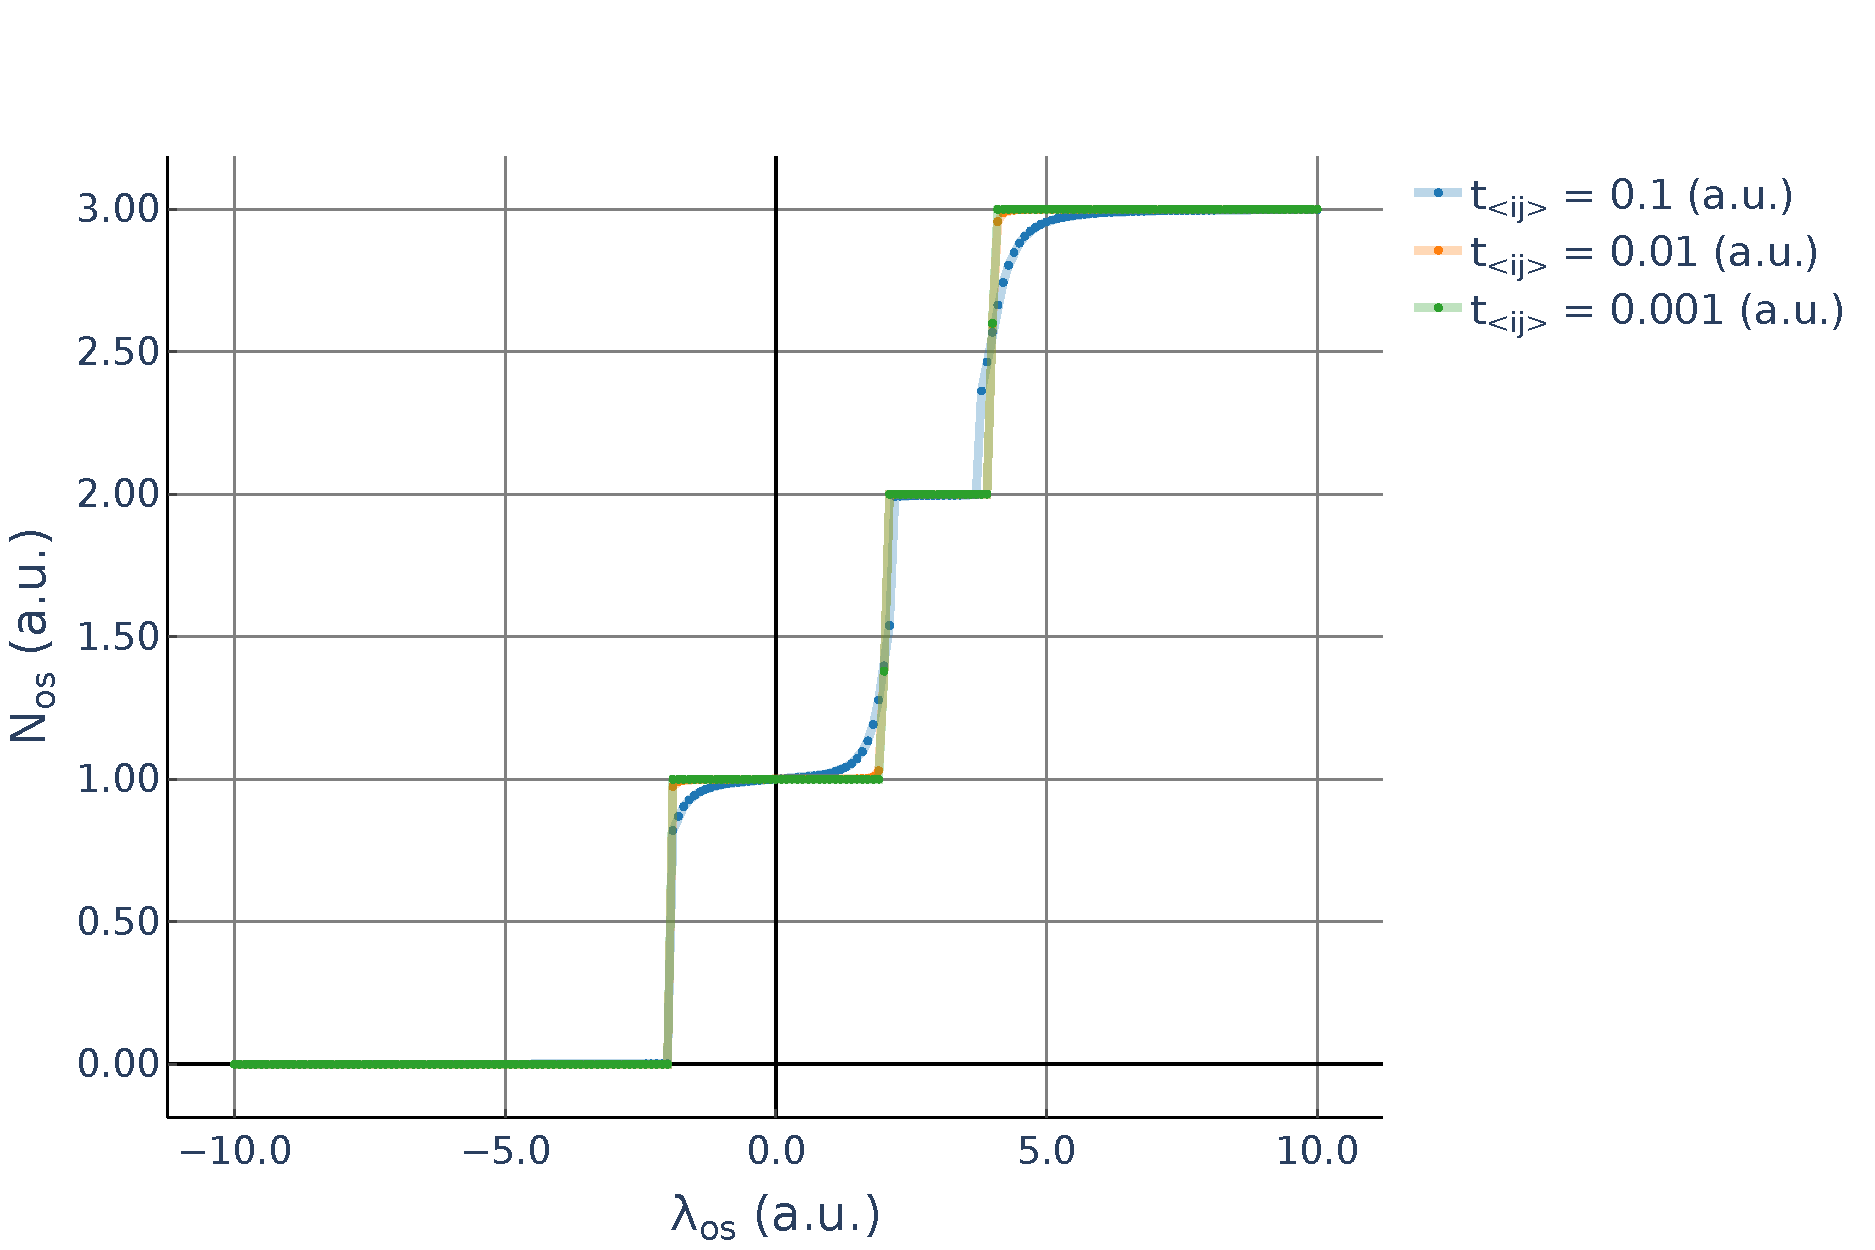
\includegraphics[width=\linewidth]{../code/figures/BH-3in3-NvsMu.pdf}
        \caption{Mott-Hubbard plateaus represented as the total open system population as a function of the applied chemical potential to the open subsystem for different values of $t_{ij}$.}
        \label{fig:Mott-Hubbard}
    \end{figure}
\end{center}
At high $U/t$, the Mott-plateaus restrict the movement of the bosons, indicating the system has transitioned to the MI-phase. The restriction of movement is also captured by the energy (\cref{fig:energetic-plateaus}), whose function becomes stepwise with energetic jumps occurring at the same critical $\mu_{os}$ where the boson-exchange takes place.
\begin{center}
  \begin{figure}
      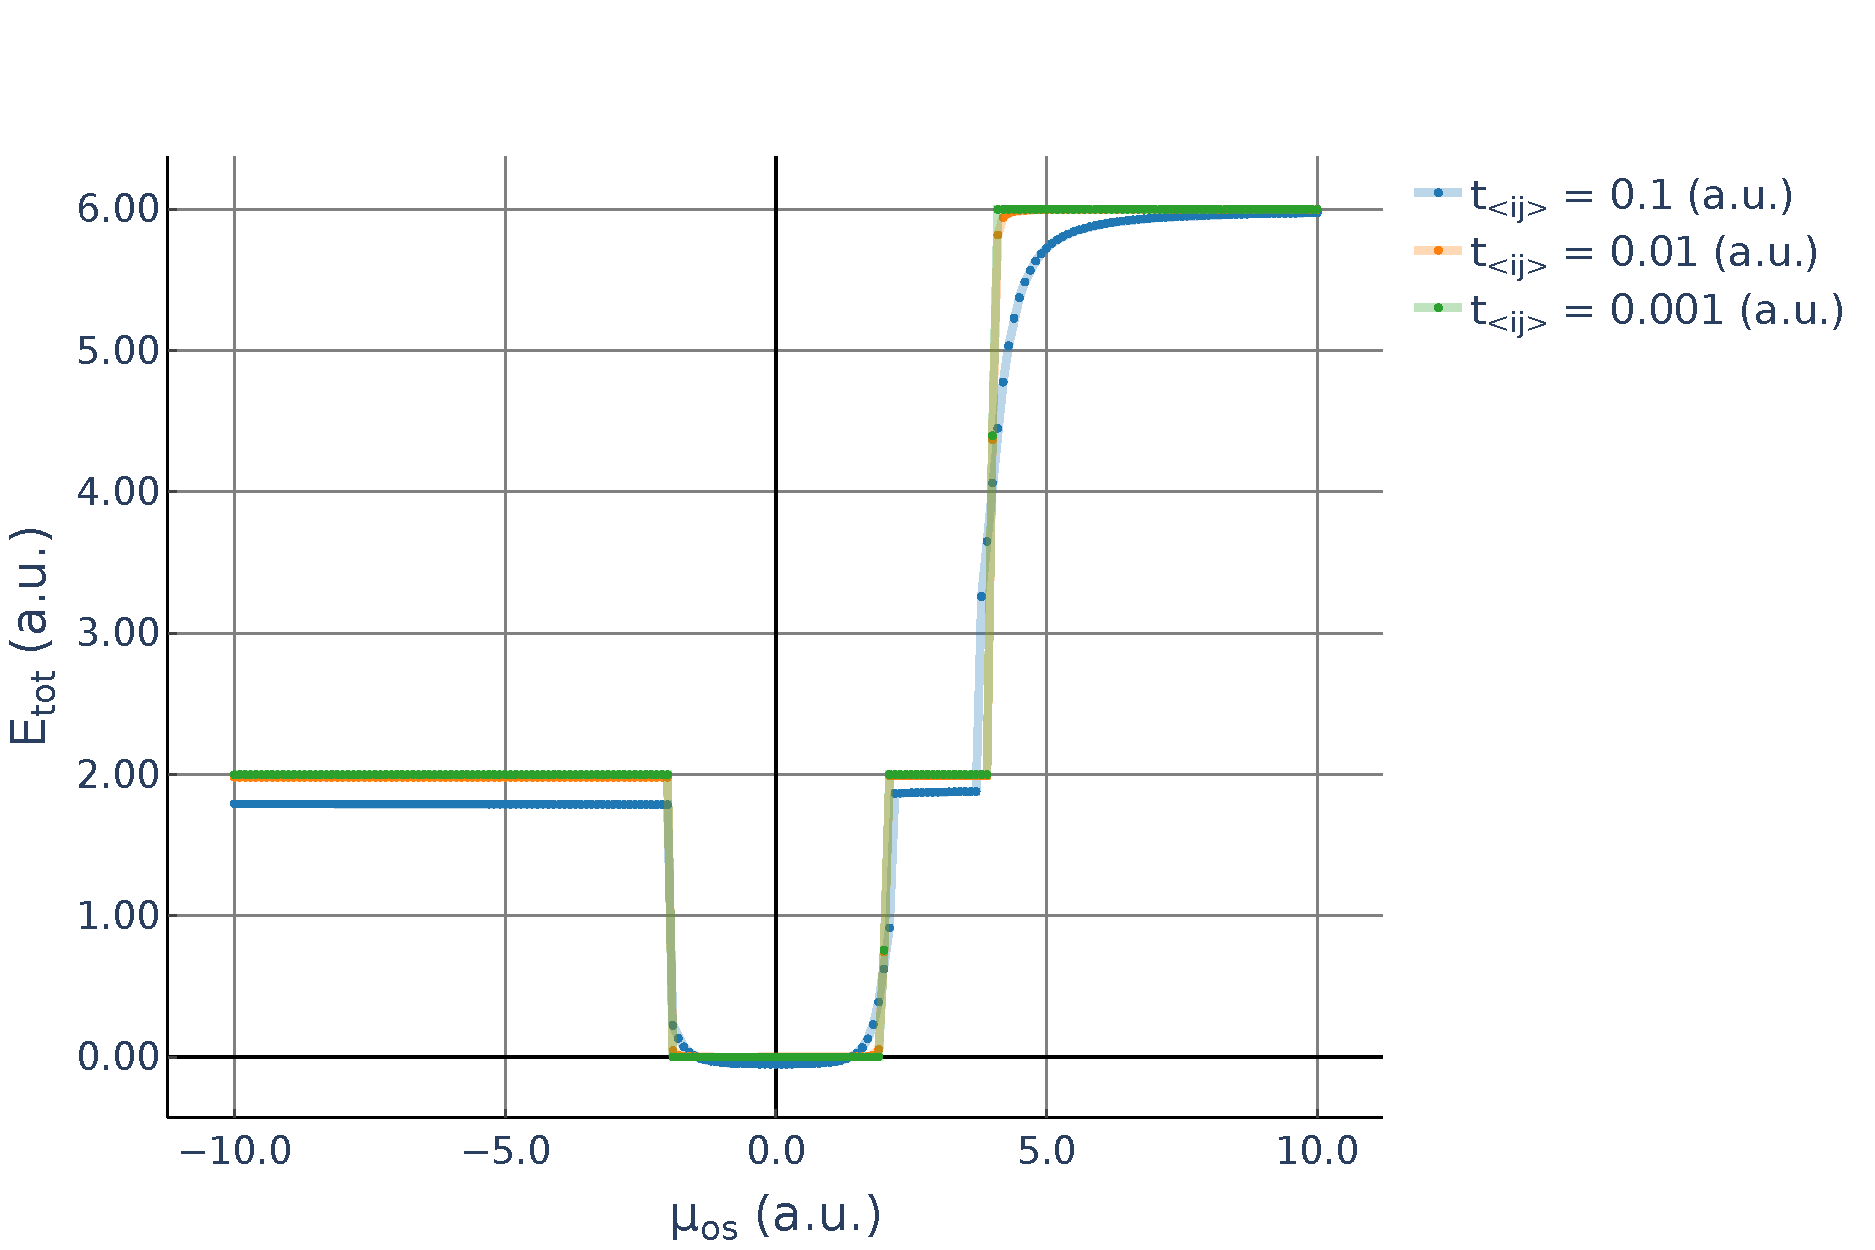
\includegraphics[width=\linewidth]{../code/figures/BH-3in3-EvsMu.pdf}
      \caption{Energetic Mott-Hubbard plateaus represented as a function of the applied chemical potential to the open subsystem for different values of $t_{ij}$.}
      \label{fig:energetic-plateaus}
  \end{figure}
\end{center}
The dual viewpoint which we can associate with these Mott-Hubbard plateaus is given by the energetic flat-planes \cite{perdew1982, cohen2008, cohen2012, yang2016}, where the total energy of the system ($E_{tot}$) becomes a series of straight line segments with discontinuities located at integer occupations (\cref{fig:flat-planes}). While previous results showed these characteristics for fermionic systems \cite{devriendt2021, devriendt2022}, we now show the same for the bosonic case.
\begin{center}
  \begin{figure}
      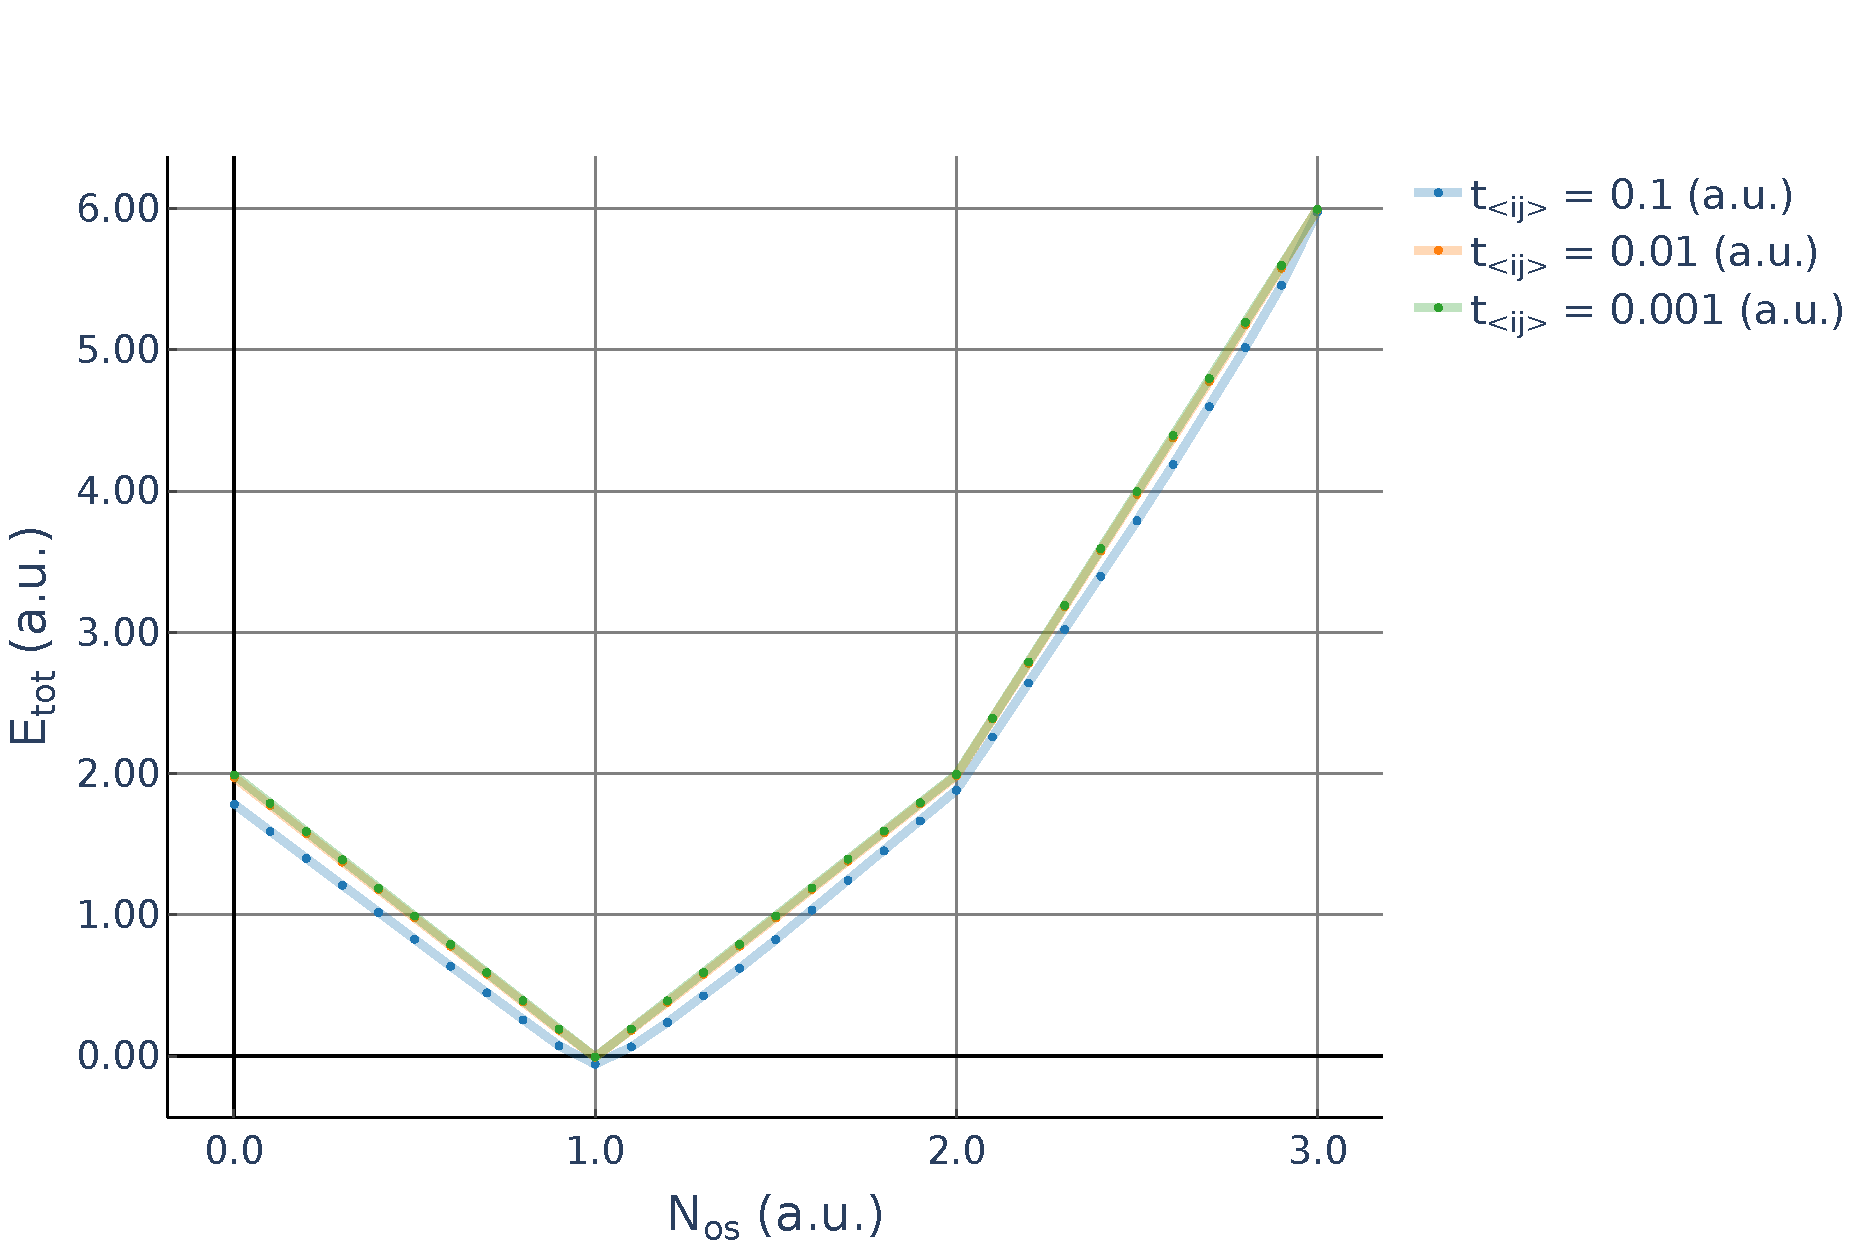
\includegraphics[width=\linewidth]{../code/figures/BH-3in3-EvsN.pdf}
      \caption{Energetic flat-planes represented by $E_{tot}$ as a function of the population of the open subsystem ($N_{os}$) for different values of $t_{ij}$.}
      \label{fig:flat-planes}
  \end{figure}
\end{center}

\subsection{DMRG can model the complete groundstate Bose-Hubbard phase diagram}

At integer filling of the sites ($\rho=\frac{N}{L}$) the one-dimensional Bose-Hubbard model describes a Mott transition (\cref{fig:Mott-Lobes}) between a so-called superfluid phase which is defined by a divergence of the momentum distribution at momentum $k$ equal to zero, and an MI phase, characterized by a finite gap for single particle excitations, defined by the difference between the potentials for half band filling and one particle less than half band filling (\cref{eq:gap}).
\begin{center}
  \begin{figure}
      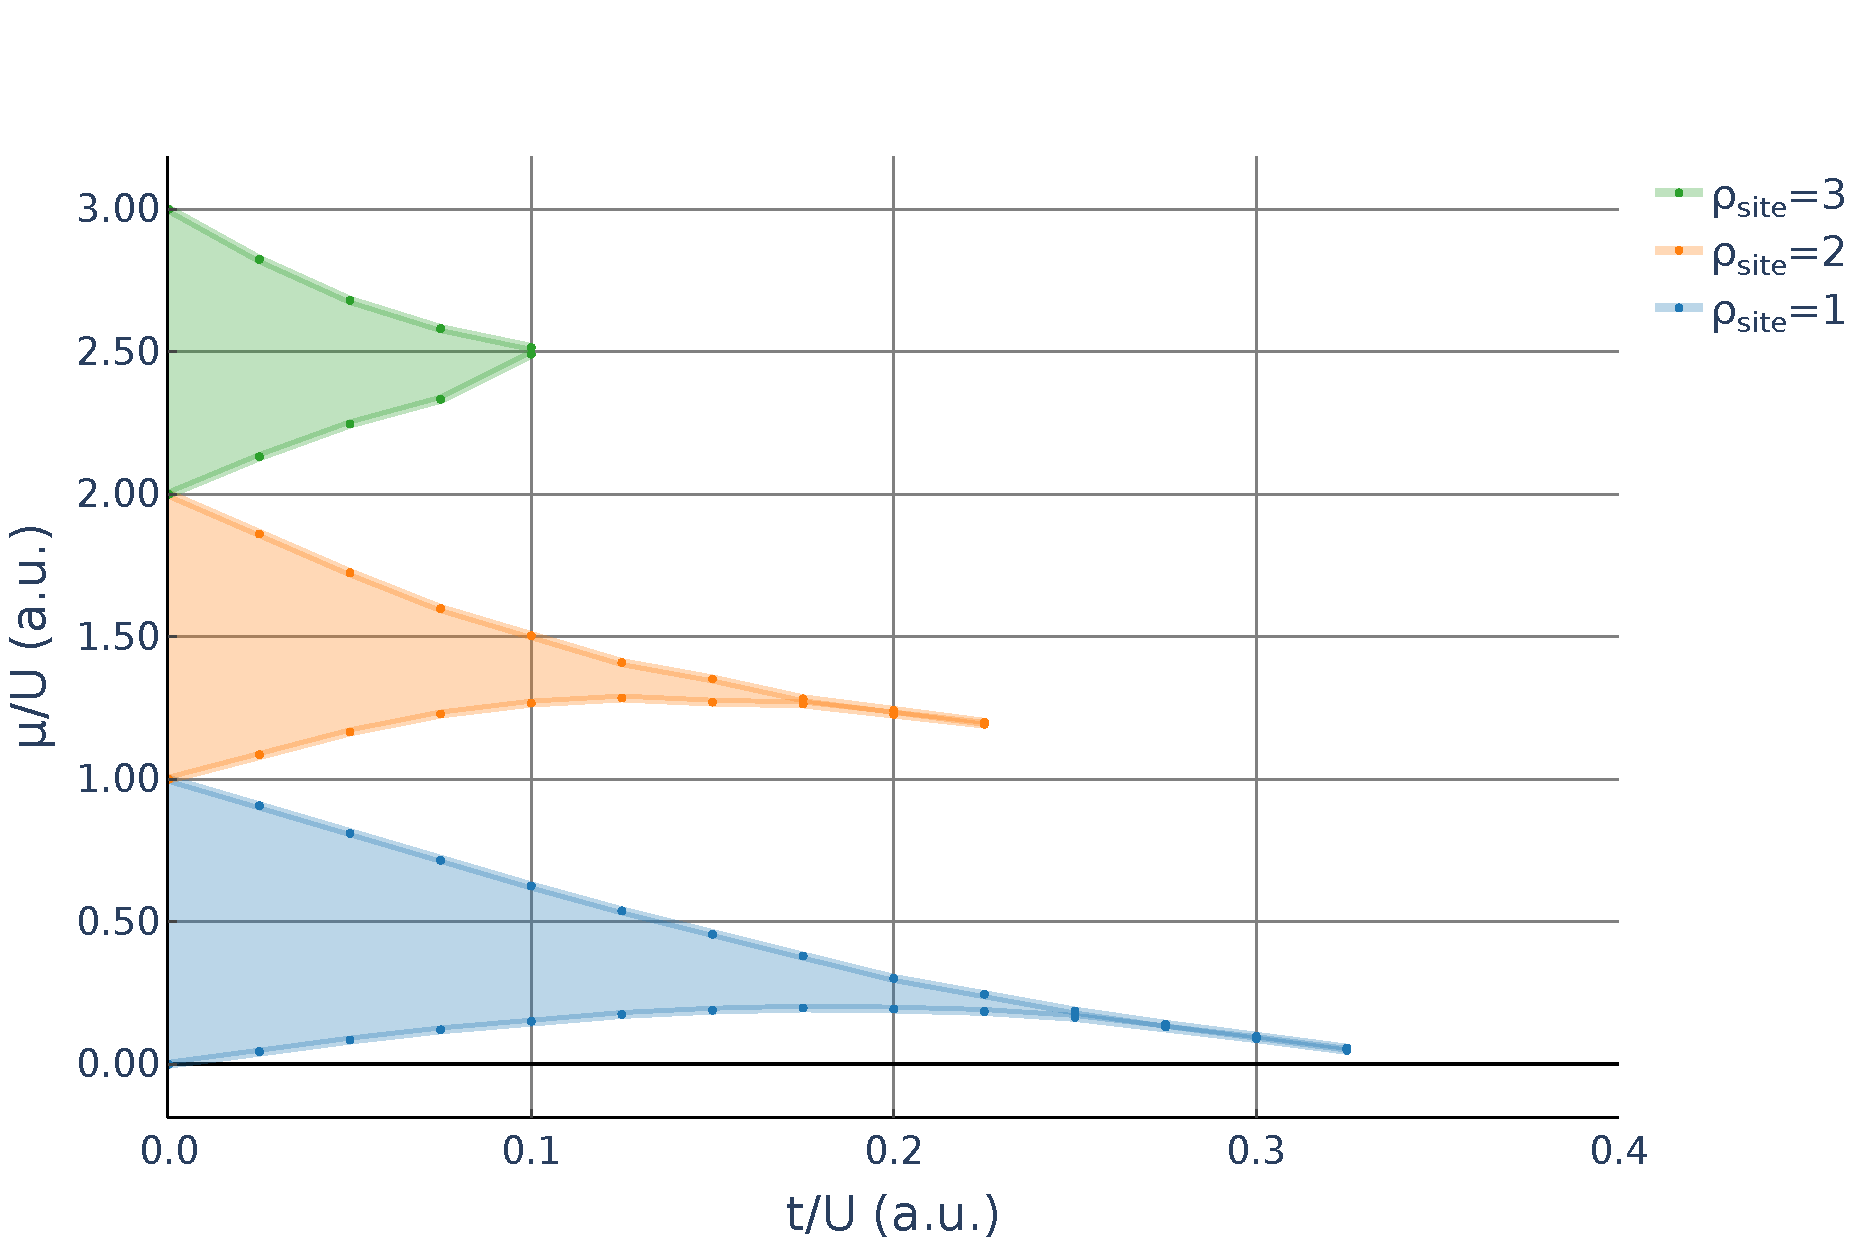
\includegraphics[width=\linewidth]{../code/figures/Mott-Lobes.pdf}
      \caption{The first three Mott Lobes of the ground state Bose-Hubbard model. Colored sections represent the MI phases, while sections outside of the boundaries represent the superfluid phase. Calculated for $L=128$ using the DMRG algorithm.}
      \label{fig:Mott-Lobes}
  \end{figure}
\end{center}
At the critical point, i.e. the tip of each Mott lobe, the model resides in the universality class of the XY-spin model, which indicates the presence of a BKT phase transition.

\section{Conclusions}

\begin{itemize}
  \item The bosonic Hubbard model shows identical characteristics to Fermi-Hubbard with the exception that multiple Mott-Hubbard plateaus arise, due to the absence of the fermionic occupation limit (i.e. Pauli's exclusion principle).
  \item The Bose Hubbard model also adheres to the flat-plane conditions as described by Perdew \cite{perdew1982}.
\end{itemize}

% \section*{Acknowledgements}

% \begin{itemize}
%   \item FWO, BOF 
%   \item HPC 
% \end{itemize}

%%%END OF MAIN TEXT%%%

%The \balance command can be used to balance the columns on the final page if desired. It should be placed anywhere within the first column of the last page.

\balance

%If notes are included in your references you can change the title from 'References' to 'Notes and references' using the following command:
%\renewcommand\refname{Notes and references}

%%%REFERENCES%%%
\bibliography{outline} %You need to replace "rsc" on this line with the name of your .bib file
\bibliographystyle{aip} %the AIP's .bst file

\end{document}
